\documentclass{beamer}

%\usepackage[noindent,nocap]{ctex}
%\usepackage[scheme=plain]{ctex}

\usepackage[style=verbose,backend=biber,maxbibnames=99,maxcitenames=1]{biblatex}
\addbibresource{slidex.bib}

%% modify fullcite definition, let it print all authors
%\preto\fullcite{\AtNextCite{\defcounter{maxnames}{99}}}

% add new command for print a publication (print all authors)
\newcommand{\printpublication}[1]{\AtNextCite{\defcounter{maxnames}{99}}\fullcite{#1}}

\usepackage{xcolor}

\usetheme{Boadilla}

\title{HPO Enrichment Analyze}
%\subtitle{}

\author{Weize Xu}
\institute{Huazhong Agriculture University}
\date{\today}
\begin{document}

\begin{frame}
\titlepage
\end{frame}

\begin{frame}
    \frametitle{Outline}
    \tableofcontents
\end{frame}

\section{Data}

\begin{frame}
    \frametitle{HPO dataset}

    The Human Phenotype Ontology (HPO)\footcite{kohler2018expansion} provides a standardized vocabulary of phenotypic abnormalities encountered in human disease. Each term in the HPO describes a phenotypic abnormality, such as Atrial septal defect.
\end{frame}

\section{Method}

\begin{frame}
    \frametitle{Enrichment}

    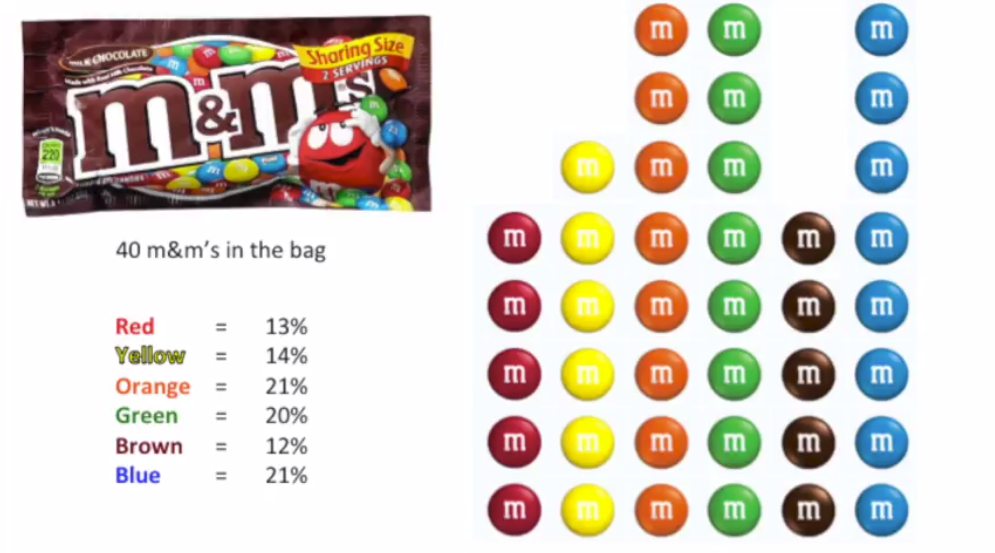
\includegraphics[scale=0.2]{mm.png}

    \footnote{https://www.youtube.com/watch?v=udyAvvaMjfM}
    
\end{frame}

\begin{frame}

    \begin{table}[]
    \begin{tabular}{lllll}
                 & succeed & failed & Total &  \\
    studying     & i       & k-i    & k     &  \\
    non-studying & m-i     &        & N-k   &  \\
    Total        & m       & N-m    & N     & 
    \end{tabular}
    \end{table}

    \frametitle{Fisher's exact test}
    The probability of hypergeometric distribution.
    \begin{equation}
        p(x=i) = \frac{ {m \choose i} { {N-m} \choose {k-i} } }{{N \choose k}}
    \end{equation}

    \begin{equation}
        pvalue = \sum_{x=i}^{k}{p(x)}
    \end{equation}
    

\end{frame}

\section{Implementation}

\begin{frame}
    \frametitle{Implementation}
    A Python package for HPO enrichment analyze.

    \small{
    \url{https://github.com/Nanguage/BioTMCourse/tree/master/HPO\%20enrich}
    }
    
\end{frame}

\begin{frame}
    \frametitle{An HPO GSEA example}

    SAGD\footcite{shi2018sagd} gene samples, SAGD\_00055(human hypothalamus tissue).

    \tiny{
    \url{https://nanguage.github.io/examples/hpo_enrich/example_sagd_00055.html}
    }
\end{frame}

\section{}

\begin{frame}
    Thank you!
\end{frame}

\section{Reference}
\begin{frame}
    \frametitle{Reference}
    \def\bibfont{\tiny}
    \printbibliography
\end{frame}

\end{document}